\documentclass[xcolor=dvipsnames]{beamer}
\usepackage[T1]{fontenc}
\usepackage[utf8]{inputenc}
\usepackage[english,slovak]{babel}

\usepackage{amsmath}
\usepackage{amsthm}
\usetheme{Pittsburgh}
\useoutertheme{shadow}

\usepackage{graphicx}
\usepackage{caption}
\usepackage{subcaption}

\usepackage[]{algorithm2e}
\usepackage{listings}
 \setbeamercovered{transparent}
 \usepackage{cuted}
\usepackage[export]{adjustbox}
\usepackage{mathtools}

\usepackage{lipsum}
\usepackage{verbatim}
\usepackage{transparent}
\usepackage{framed}
\usepackage{xcolor}

\usepackage{multirow}
\usepackage{colortbl}
\usepackage{lmodern}

\usepackage{movie15}
\usepackage{media9}
\usepackage{verbatim}

\usepackage{animate}


\usepackage{hyperref}

\newcommand\Wider[2][3em]{%
\makebox[\linewidth][c]{%
  \begin{minipage}{\dimexpr\textwidth+#1\relax}
  \raggedright#2
  \end{minipage}%
  }%
}






\iftrue

\usetheme{Warsaw}

\setbeamercolor{normal text}{fg=white,bg=black!90}
\setbeamercolor{structure}{fg=white}

\setbeamercolor{alerted text}{fg=red!85!black}

\setbeamercolor{item projected}{use=item,fg=black,bg=item.fg!35}

\setbeamercolor*{palette primary}{use=structure,fg=structure.fg}
\setbeamercolor*{palette secondary}{use=structure,fg=structure.fg!95!black}
\setbeamercolor*{palette tertiary}{use=structure,fg=structure.fg!90!black}
\setbeamercolor*{palette quaternary}{use=structure,fg=structure.fg!95!black,bg=black!80}

\setbeamercolor*{framesubtitle}{fg=white}

\setbeamercolor*{block title}{parent=structure,bg=black!60}
\setbeamercolor*{block body}{fg=black,bg=black!10}
\setbeamercolor*{block title alerted}{parent=alerted text,bg=black!15}
\setbeamercolor*{block title example}{parent=example text,bg=black!15}

\fi



%-------------------------------------------------------------------------------------
\title{\color{white} \bf random network distillation}
\author{\color{white} Michal CHOVANEC, PhD}


%\setbeamertemplate{footline}[frame number]{}
\setbeamertemplate{navigation symbols}{}


\date[EURP]{}
\begin{document}

{
    \usebackgroundtemplate
    {
        \vbox to \paperheight{\vfil\hbox to \paperwidth{\hfil

        {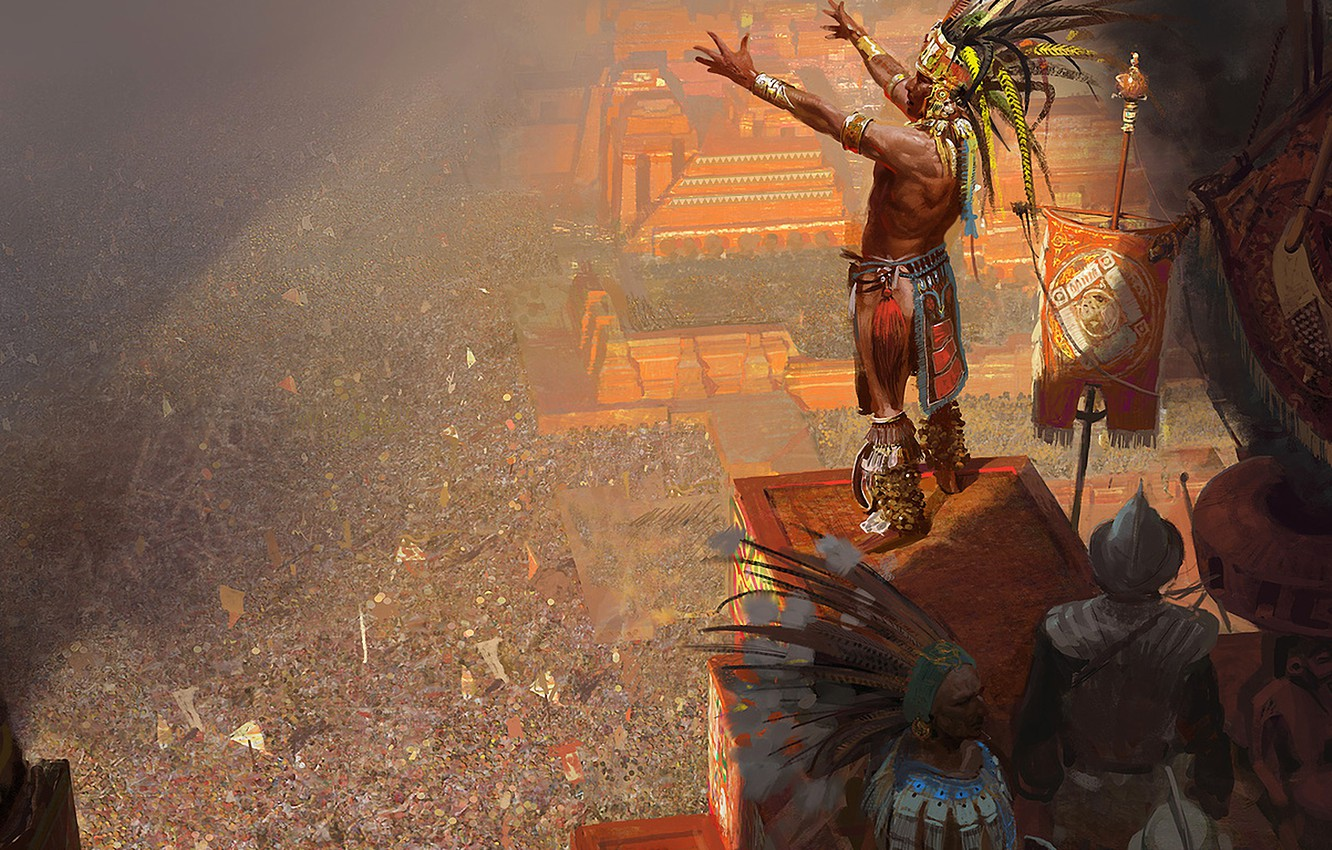
\includegraphics[width=5.05in]{../images/aztec.jpg}}

        \hfil}\vfil}
    }

    \begin{frame}
     \centering
     {
        \begin{minipage}{10cm}
           {\LARGE \color{white}{\bf challenging Montezuma's Revenge}} \\
           {\LARGE \color{white}{\bf intrinsic motivation in RL}} \\
           {\LARGE \color{white}{\bf Michal CHOVANEC}} \\
       \end{minipage}
     }

    \end{frame}
}


\begin{frame}{\bf loss}

  \begin{align*}
    \mathcal{L(\theta)} = &(R_a^{ext} - V_a^{ext}(\theta))^2 + (R_a^{int} - V_a^{int}(\theta))^2 + \\
    &(R_b^{ext} - V_b^{ext}(\theta))^2 + (R_b^{int} - V_b^{int}(\theta))^2 + \\
    &-\frac{\pi_a^{\theta}(a_a | s,g)} {\pi_a^{\theta'}(a_a | s,g)} A_{a} - \frac{\pi_b^{\theta}(a_b | s,g)} {\pi_b^{\theta'}(a_b | s,g)} A_{b} + \\
    &\eta H(\pi_a^{\theta}) + \eta H(\pi_b^{\theta})
  \end{align*} 
 
\end{frame}





\end{document}
